\normaltrue \difficilefalse \tdifficilefalse
\correctionfalse

%\UPSTIidClasse{11} % 11 sup, 12 spé
%\newcommand{\UPSTIidClasse}{12}

\exer{EPAS $\star$ \label{B2:10:64}}
\setcounter{numques}{0}
\UPSTIcompetence[2]{B2-10}
\index{Compétence B2-10}
\index{EPAS}
\ifcorrection
\else
\textbf{Pas de corrigé pour cet exercice.}
\fi

\ifprof
\else


On s'intéresse à l'échelle pivotante équipant un camion de pompier.

\begin{figure}[H]
\centering
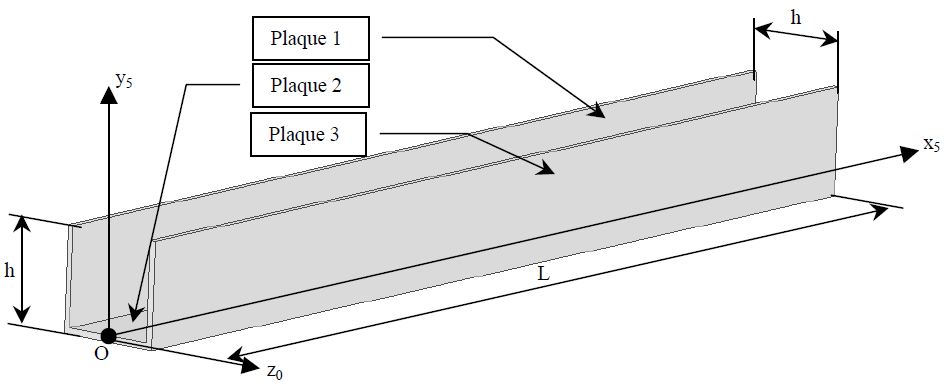
\includegraphics[width=\linewidth]{64_01}
\end{figure}

Les deux vérins doivent être capables de déplacer l’ensemble du parc échelle et la plate-forme
chargée.

\textbf{Le parc échelle (5) :} 
on notera la matrice d’inertie du parc échelle au point $G$ (son centre de gravité) dans la base 
$\base{x_5}{y_5}{z_0}$ : $\inertie{G}{5} = \matinertie{I_{Gx}}{I_{Gy}}{I_{Gz}}{0}{0}{0}{\base{x_5}{y_5}{z_0}}$. Le parc échelle a une masse notée $3m$ et une longueur notée $L$. Son centre de gravité $G$ est tel que $\vect{OG}=\dfrac{L}{2}\vect{x_5}+\dfrac{h}{3}\vect{y_5}$. 
Le parc échelle est solidaire du berceau avec $\vect{OA}=d\vect{x_5}$

\textbf{La plate forme chargée (6):} pendant le redressement ou l’abaissement, la plate-forme reste toujours horizontale.
Sa masse une fois chargée sera notée $M$ et son centre de gravité est le point $G_P$ tel que : 
$\vect{DG_P}=\lambda \vect{x_0} + \mu\vect{y_0}$.
On notera la matrice d’inertie de la plate forme chargée au point $G_P$ (son centre de gravité) dans la base 
$\base{x_0}{y_0}{z_0}$ : $\inertie{G_P}{6} = \matinertie{A}{B}{C}{0}{0}{0}{\base{x_0}{y_0}{z_0}}$.

\textbf{Le berceau (5) :} sa masse sera négligée devant les autres masses. Il est incliné par rapport à l’horizontal d’un angle $\theta$ fonction du temps.

\textbf{Les vérins (3+4) :} leurs masses seront négligées devant les autres masses.
Ils devront exercer un effort, modélisé par un glisseur de résultante $\vect{R}=R\vy{3}$ , permettant le
déplacement $\theta$.
\fi

\question{Déterminer l’expression littérale du moment dynamique en $A$ de l’ensemble
\{parc échelle + berceau\} \textbf{(5)} par rapport au châssis \textbf{(0)} : $\vectmd{A}{5}{0}$.}
\ifprof
\else
\fi

\question{Déterminer l’expression littérale du moment dynamique en $A$ de la plate-forme
\textbf{(6)} par rapport au châssis \textbf{(0)} : $\vectmd{A}{6}{0}$.}
\ifprof
\else
\fi

\question{Déterminer l’expression littérale de l’effort $R$ que devra fournir l’ensemble des
deux vérins sur le berceau, en fonction des masses, des paramètres géométriques et de l’angle
$\theta$ et de ses dérivées. Indiquer clairement les sous-ensembles isolés, les actions mécaniques
prises en compte et les théorèmes utilisés.}
\ifprof
\else
\fi



\ifprof
\footnotesize
\begin{itemize}
\item $\vectmd{A}{5}{0} = \left[I_{Gz}+3m\left[\left(\dfrac{L}{2}-d\right)^2+\dfrac{h^2}{9}\right]\right]\ddot{\theta}\vz{0}$.
\item $\vectmd{A}{6}{0} = M\left[H\ddot{\theta}\left(H+\lambda\cos\theta +\mu\sin\theta\right) +H\dot{\theta}^2\left( -\lambda \sin \theta + \mu \cos\theta \right) \right]\vz{0}$.
\item $R = \dfrac{
\left[I_{Gz}+3m \left[ \left(\dfrac{L}{2} -d\right)^2+\dfrac{h^2}{9}\right] \right]\ddot{\theta}
+M\left[H\ddot{\theta}\left(H+\lambda\cos\theta +\mu\sin\theta\right) +H\dot{\theta}^2\left( -\lambda \sin \theta + \mu \cos\theta \right) \right]
+3mg \left[ \left(\dfrac{L}{2} -d\right)\cos\theta+\dfrac{h}{3} \sin\theta\right] 
+Mg\left[H\cos\theta + \lambda \right]
}{c\cos\left(\theta-\beta\right)}$.
\end{itemize}
\normalsize
\else
\begin{flushright}
\footnotesize{Corrigé voir \ref{B2:10:64}.}
\end{flushright}%
\fi